\section{Resultados y Análisis}
\subsection{Software}
\begin{frame}[t]
\frametitle{Resultados y Análisis}
\framesubtitle{Aplicación Web}

	\begin{figure}[!]
		\centering
		\caption{Vista Usuario Administrador. [Imagen Propia]}
		\label{fig:adminview}
		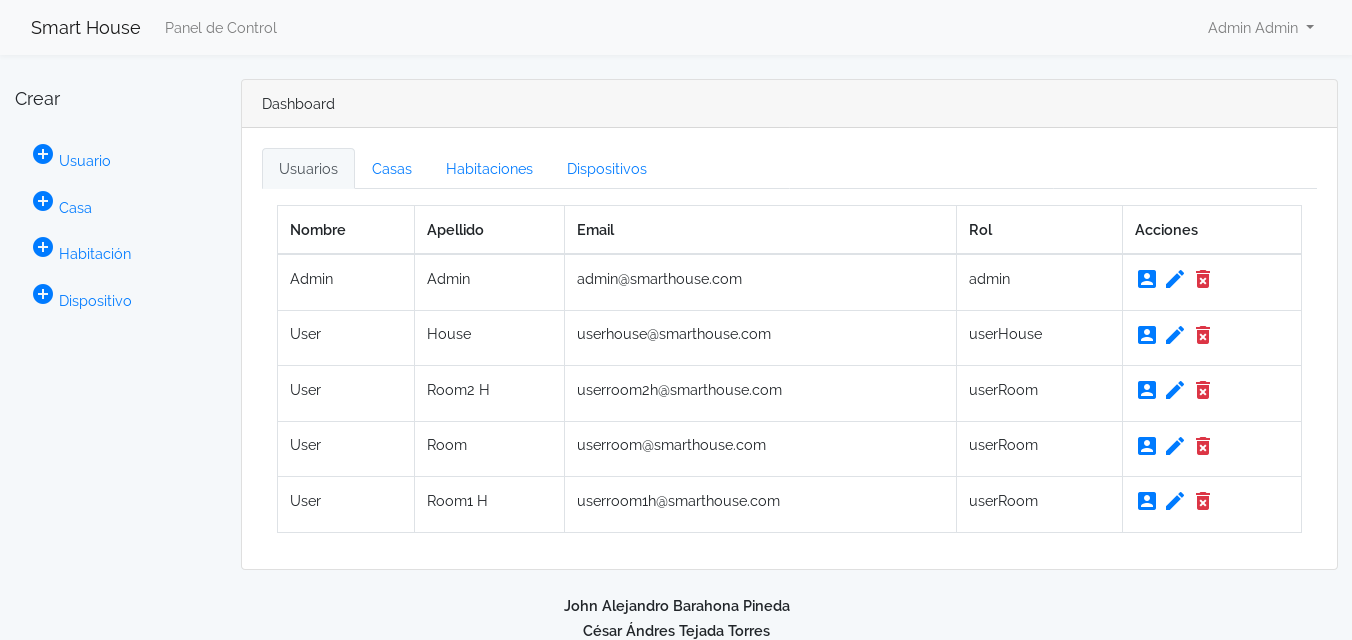
\includegraphics[width=\linewidth]{Imagenes/Admin_view}
	\end{figure}

\end{frame}	

\begin{frame}[t]
\frametitle{Resultados y Análisis}
\framesubtitle{Aplicación Web}
	
	\begin{figure}[!]
		\centering
		\caption{Vista Usuario de Casa. [Imagen Propia]}
		\label{fig:houseview}
		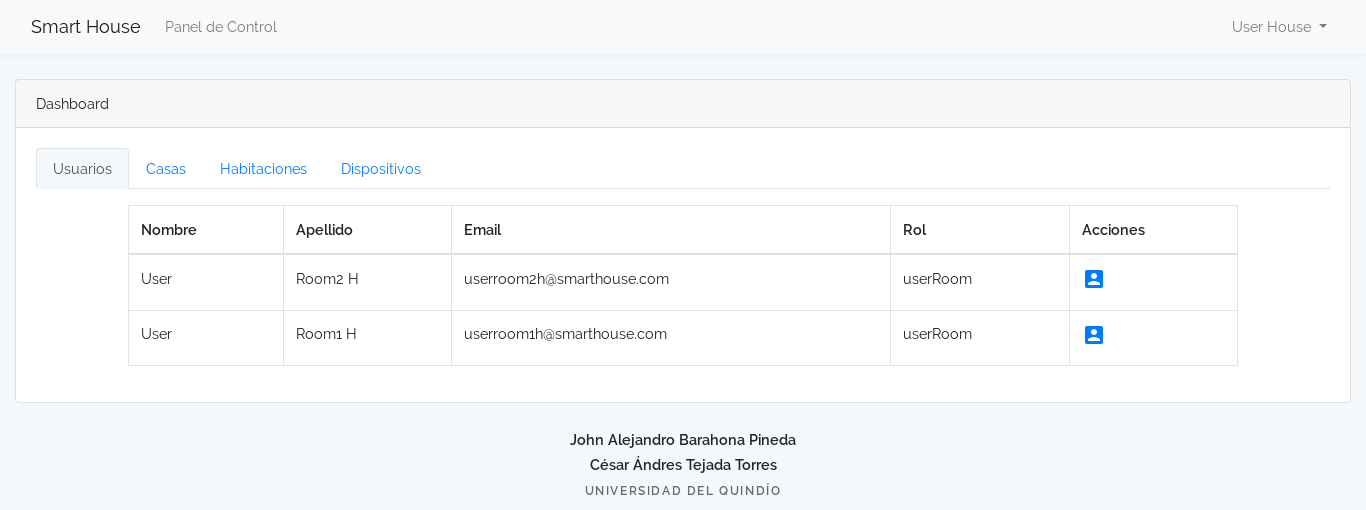
\includegraphics[width=\linewidth]{Imagenes/UserH_view}
	\end{figure}

\end{frame}

\begin{frame}[t]
\frametitle{Resultados y Análisis}
\framesubtitle{Aplicación Web}
\begin{columns}[t]
	\column[t]{0.6\linewidth}
	\begin{figure}[!]
		\centering
		\caption{Vistas de Usuario Habitación [Imagen Propia]}
		\label{fig:userview}
		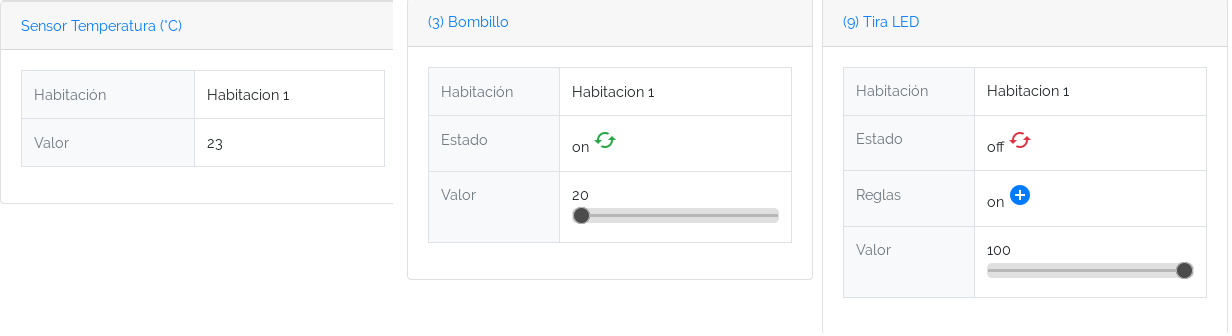
\includegraphics[width=\linewidth]{Imagenes/R_App}
	\end{figure}

	\column[t]{0.4\linewidth}
	\begin{figure}[!]
		\centering
		\caption{Vista para añadir reglas [Imagen Propia]}
		\label{fig:rulesview}
		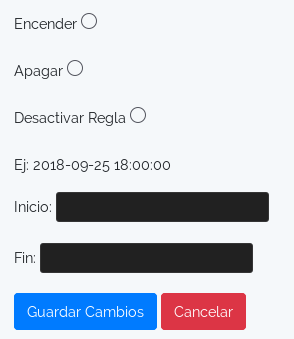
\includegraphics[width=0.7\linewidth]{Imagenes/rules_view}
	\end{figure}
\end{columns}
\end{frame}

\subsubsection{Base de Datos}
\begin{frame}
\frametitle{Resultados y Análisis}
\framesubtitle{Software | \emph{Base de Datos}}
\begin{figure}[H]
\centering
\caption{Base de datos SmartHouse [Imagen Propia]}
\label{fig:db}
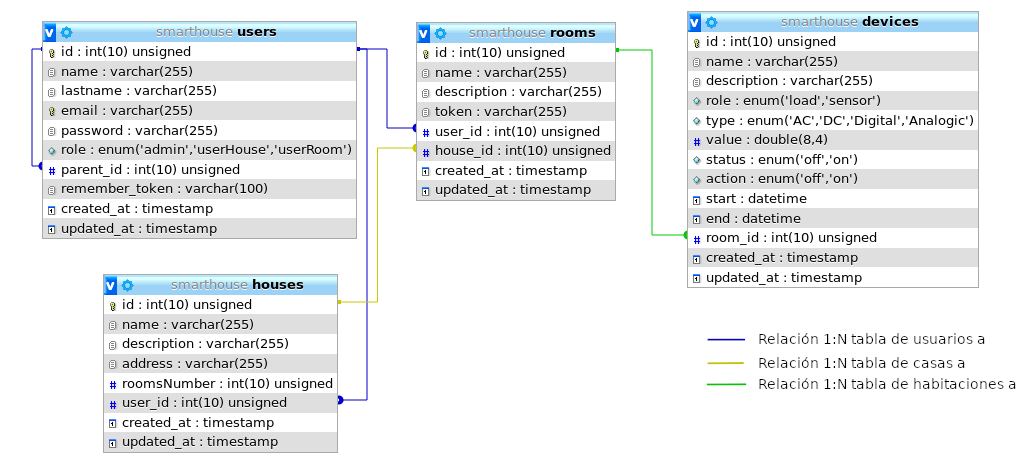
\includegraphics[width=0.75\linewidth]{Imagenes/DB}
\end{figure}

\end{frame}


\subsection{Firmware}
\begin{frame}
\frametitle{Resultados y Análisis}
\framesubtitle{Aplicación Sistema Embebido}
\begin{columns}
	\column[t]{0.5\linewidth}
\begin{figure}
	\centering
	\caption{Conexión a Internet vía Wi-Fi ESP32 [Imagen Propia]}
	\label{fig:conexion}
	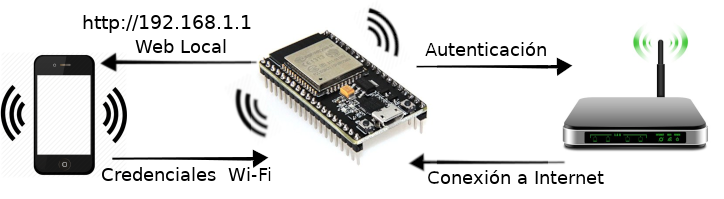
\includegraphics[width=\linewidth]{Imagenes/conexion}
\end{figure}
	\column[t]{0.5\linewidth}

\begin{table}[H]
	\begin{center}
		\caption{Resumen Aplicación.}
	\begin{tabular}{|c|c|}
		\hline 
		Tareas & 12 \\ 
		\hline 
		Interrupciones & 3 \\
		\hline
		Timers & 2 \\ 
		\hline 
		Memoria heap disponible & 160KB \\ 
		\hline 
		Tiempo petición HTTP & 1s \\ 
		\hline 
	\end{tabular} 
\end{center}
\end{table}
	
\end{columns}
\end{frame}

\subsection{Hardware}
\begin{frame}[t]
\frametitle{Resultados y Análisis}
\framesubtitle{Hardware}
\begin{columns}
	\column[t]{0.6\linewidth}
\begin{figure}
	\centering
	\caption{Tarjeta SmartHouse [Imagen Propia]}
	\label{fig:tarjeta}
	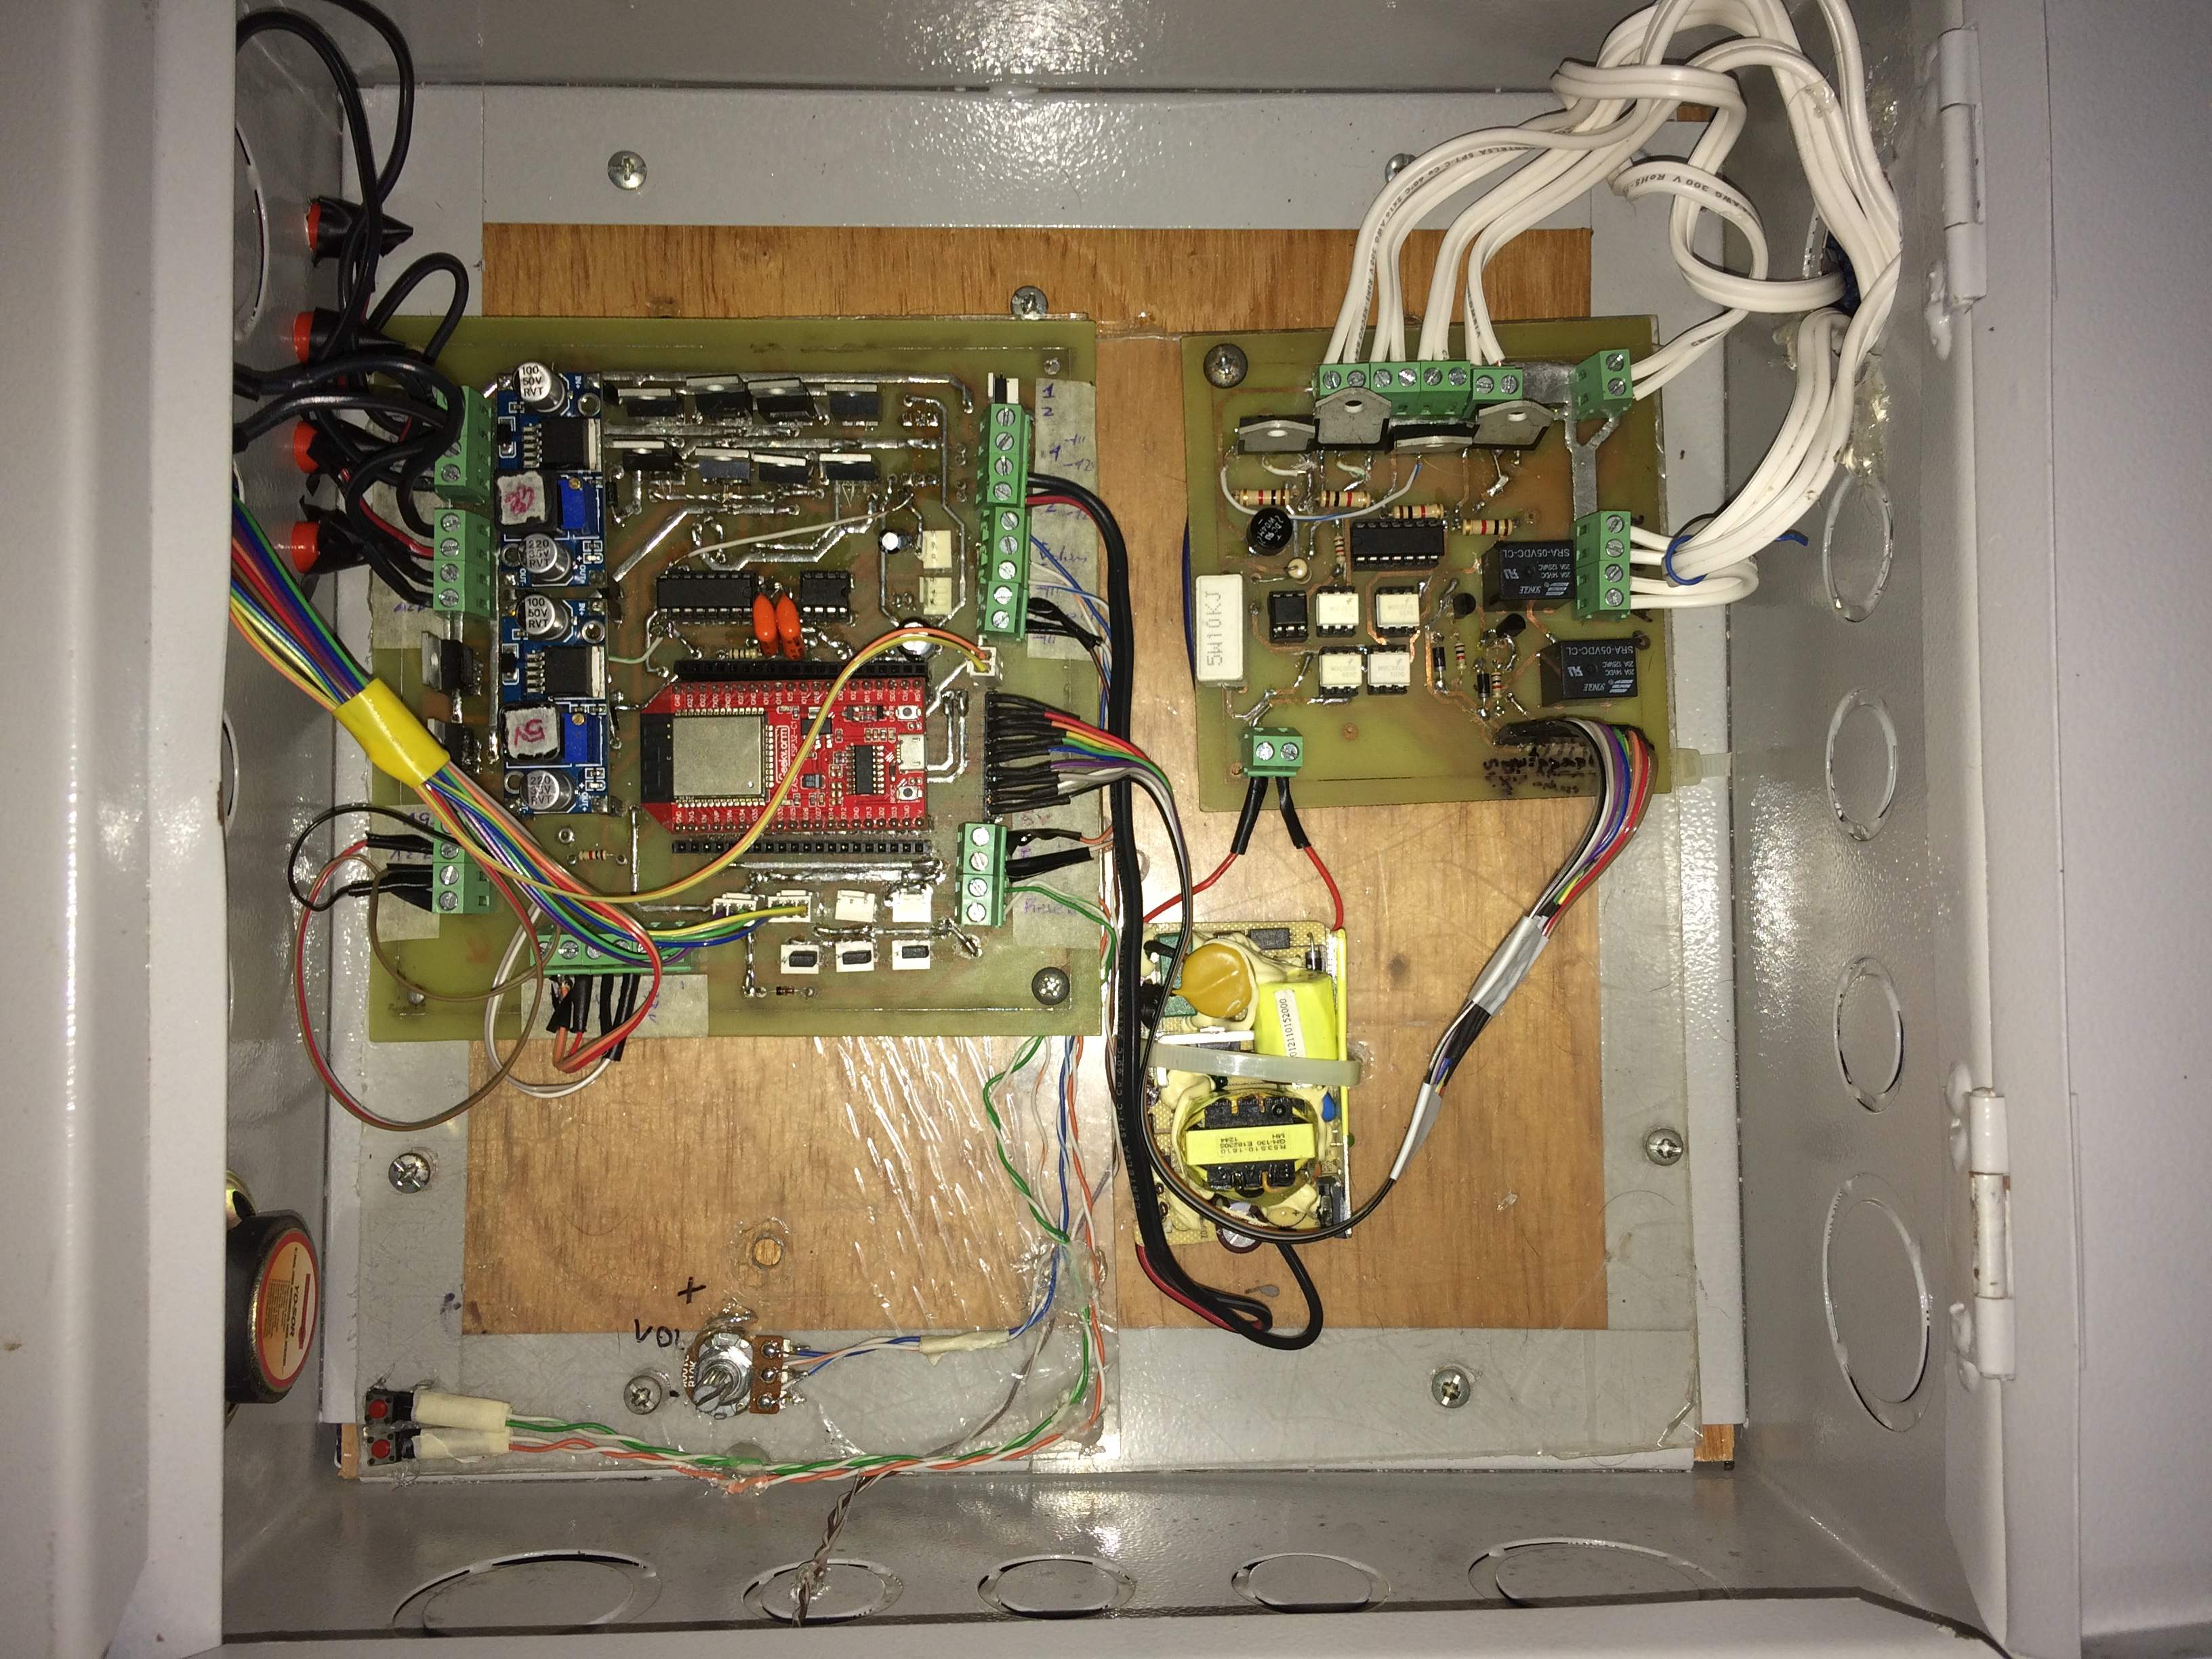
\includegraphics[width=\linewidth]{Imagenes/Tarjeta.jpg}
\end{figure}
	\column[t]{0.35\linewidth}
\begin{figure}
	\centering
	\caption{Tarjeta SmartHouse [Imagen Propia]}
	\label{fig:caja}
	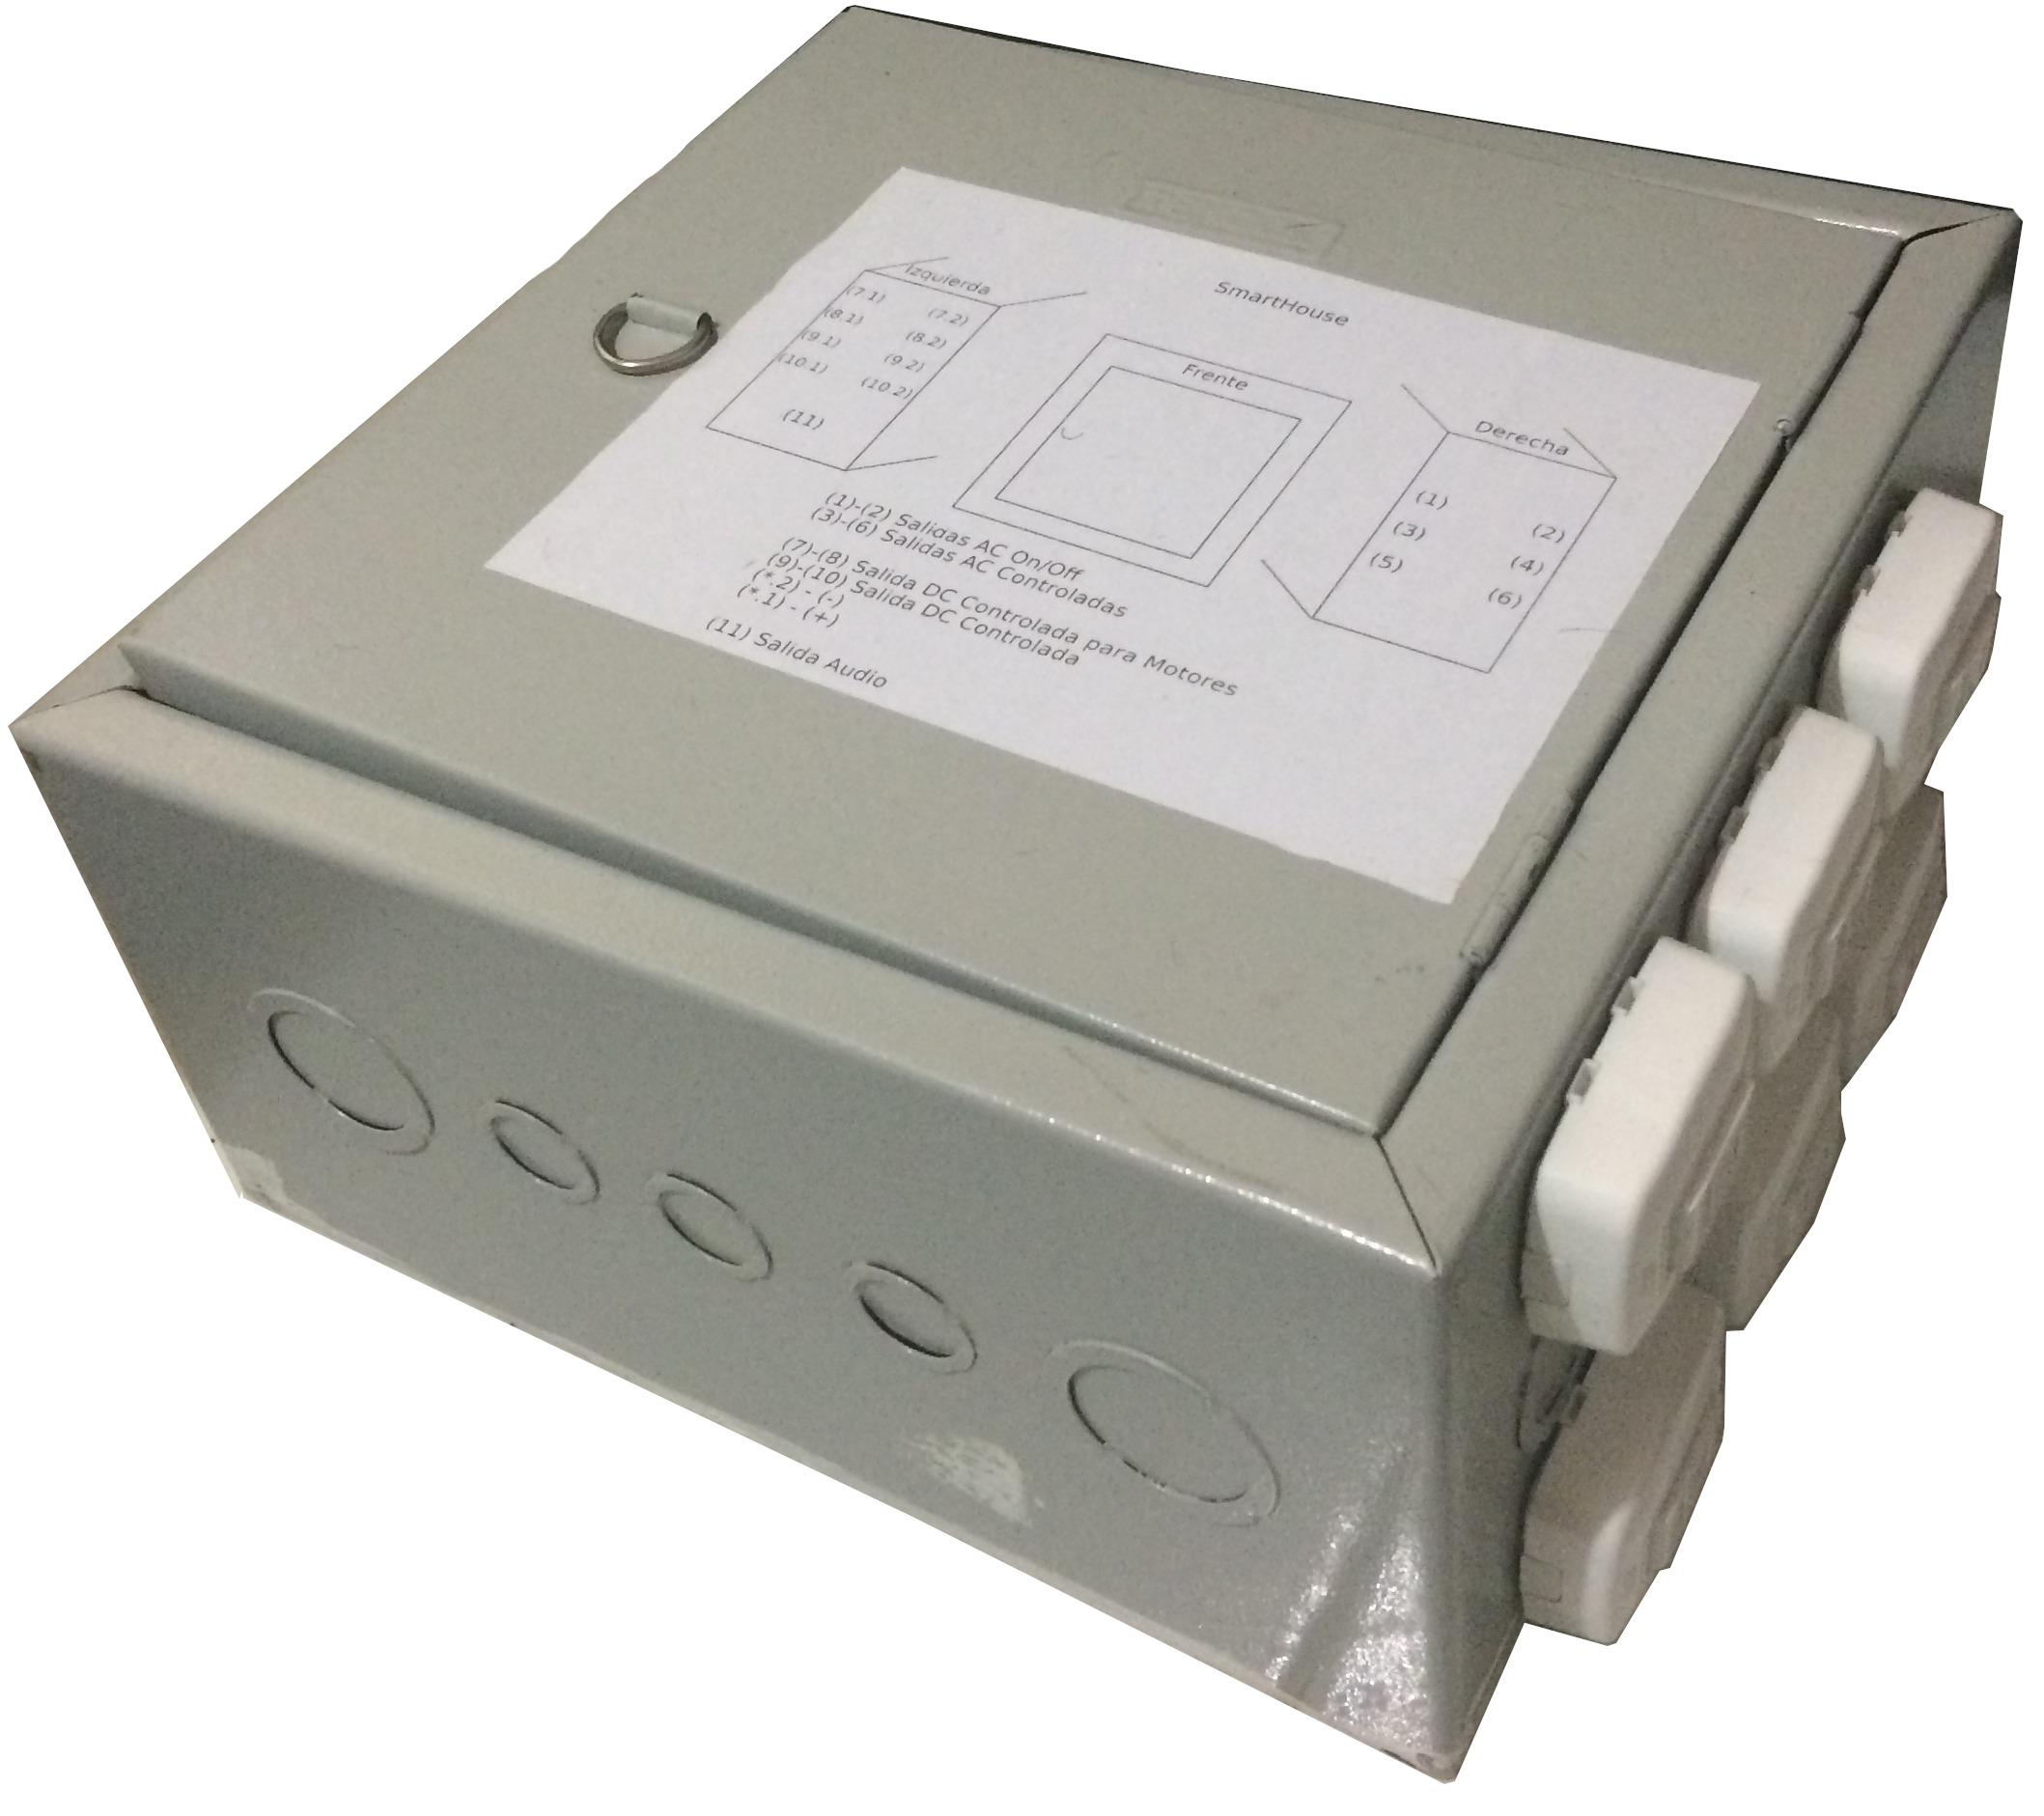
\includegraphics[width=\linewidth]{Imagenes/caja.jpg}
\end{figure}
\end{columns}
\end{frame}

\subsection{Prueba Beta Cerrada}
\begin{frame}[t]
\frametitle{Resultados y Análisis}
\framesubtitle{Prueba Beta Cerrada}
\footnotesize 
\begin{columns}
	\column{\dimexpr\paperwidth-10pt}
\begin{table}[H]
	\begin{center}
		\caption{Resultados por pregunta.}
		\label{table:enc}
		\begin{tabular}{|p{11cm}|c|c|}
			\hline 
			\textbf{Número de la Pregunta} & \textbf{Promedio} & \textbf{Desv. Est.}\\ 
			\hline 
			{\tiny El método para conectar la tarjeta a Internet por medio de Wi-Fi es sencillo de realizar.} & 4.5 & 0.52\\ 
			\hline 
			{\tiny La interfaz para seleccionar la red e ingresar las credenciales es fácil de utilizar.} & 4.8 & 0.41\\ 
			\hline 
			{\tiny En caso del cambio de nombre o contraseña de su red Wi-Fi, es fácil volver a configurar la tarjeta para que esta se conecte de nuevo.} & 4.5 & 0.74\\ 
			\hline 
			{\tiny El inicio de sesión en la pagina web es claro.} & 5.0 & 0.00\\ 
			\hline 
			{\tiny En la aplicación web, los datos de los sensores y estados de las salidas se presentan de una manera clara y entendible.} & 4.9 & 0.35\\ 
			\hline 
			{\tiny Encender o apagar un dispositivo o salida es sencillo y se presenta de forma clara.} & 4.9 & 0.35\\ 
			\hline 
			{\tiny El tiempo de respuesta después de encender o apagar un dispositivo desde la aplicación es bueno.} & 4.3 & 0.80\\ 
			\hline 
			{\tiny Las reglas para los dispositivos o salidas son fáciles de configurar y eliminar.} & 4.3 & 0.82\\ 
			\hline 
			{\tiny La aplicación web es fácil de usar.} & 4.8 & 0.41\\ 
			\hline 
			\textbf{Total} & \textbf{4.7} & \textbf{0.24}\\ 
			\hline 
		\end{tabular} 
	\end{center}
\end{table}
\end{columns}

\end{frame}